\chapter{Repair of 922 Lynx master} \label{app:922repair}
In early February 2017, the piezo actuator on the 922 shorted. 
I suspect it just got old or the Sacher driver killed it but whatever the cause we ordered a new one from Sacher (also ordered a spare which I put in the blue and beige cabinet in the Neutral lab). 
As of March 1st 2017 it seems that the 922 master is back up and running without issue. 

The images below are how I changed the PZT. 
There was originally some more epoxy around the brass cup but Tom chipped that away so we could unscrew the cup from the flexure arm, this is what holds the PZT.
The only other tricky part is removing the back circuit board to get access to the spring terminals that face down.
Once you get access here replacing the PZT is fairly trivial.

I also include, at the end, a letter we received from Sacher once they sent us the new PZTs.
	\begin{figure}
		\centerline{
		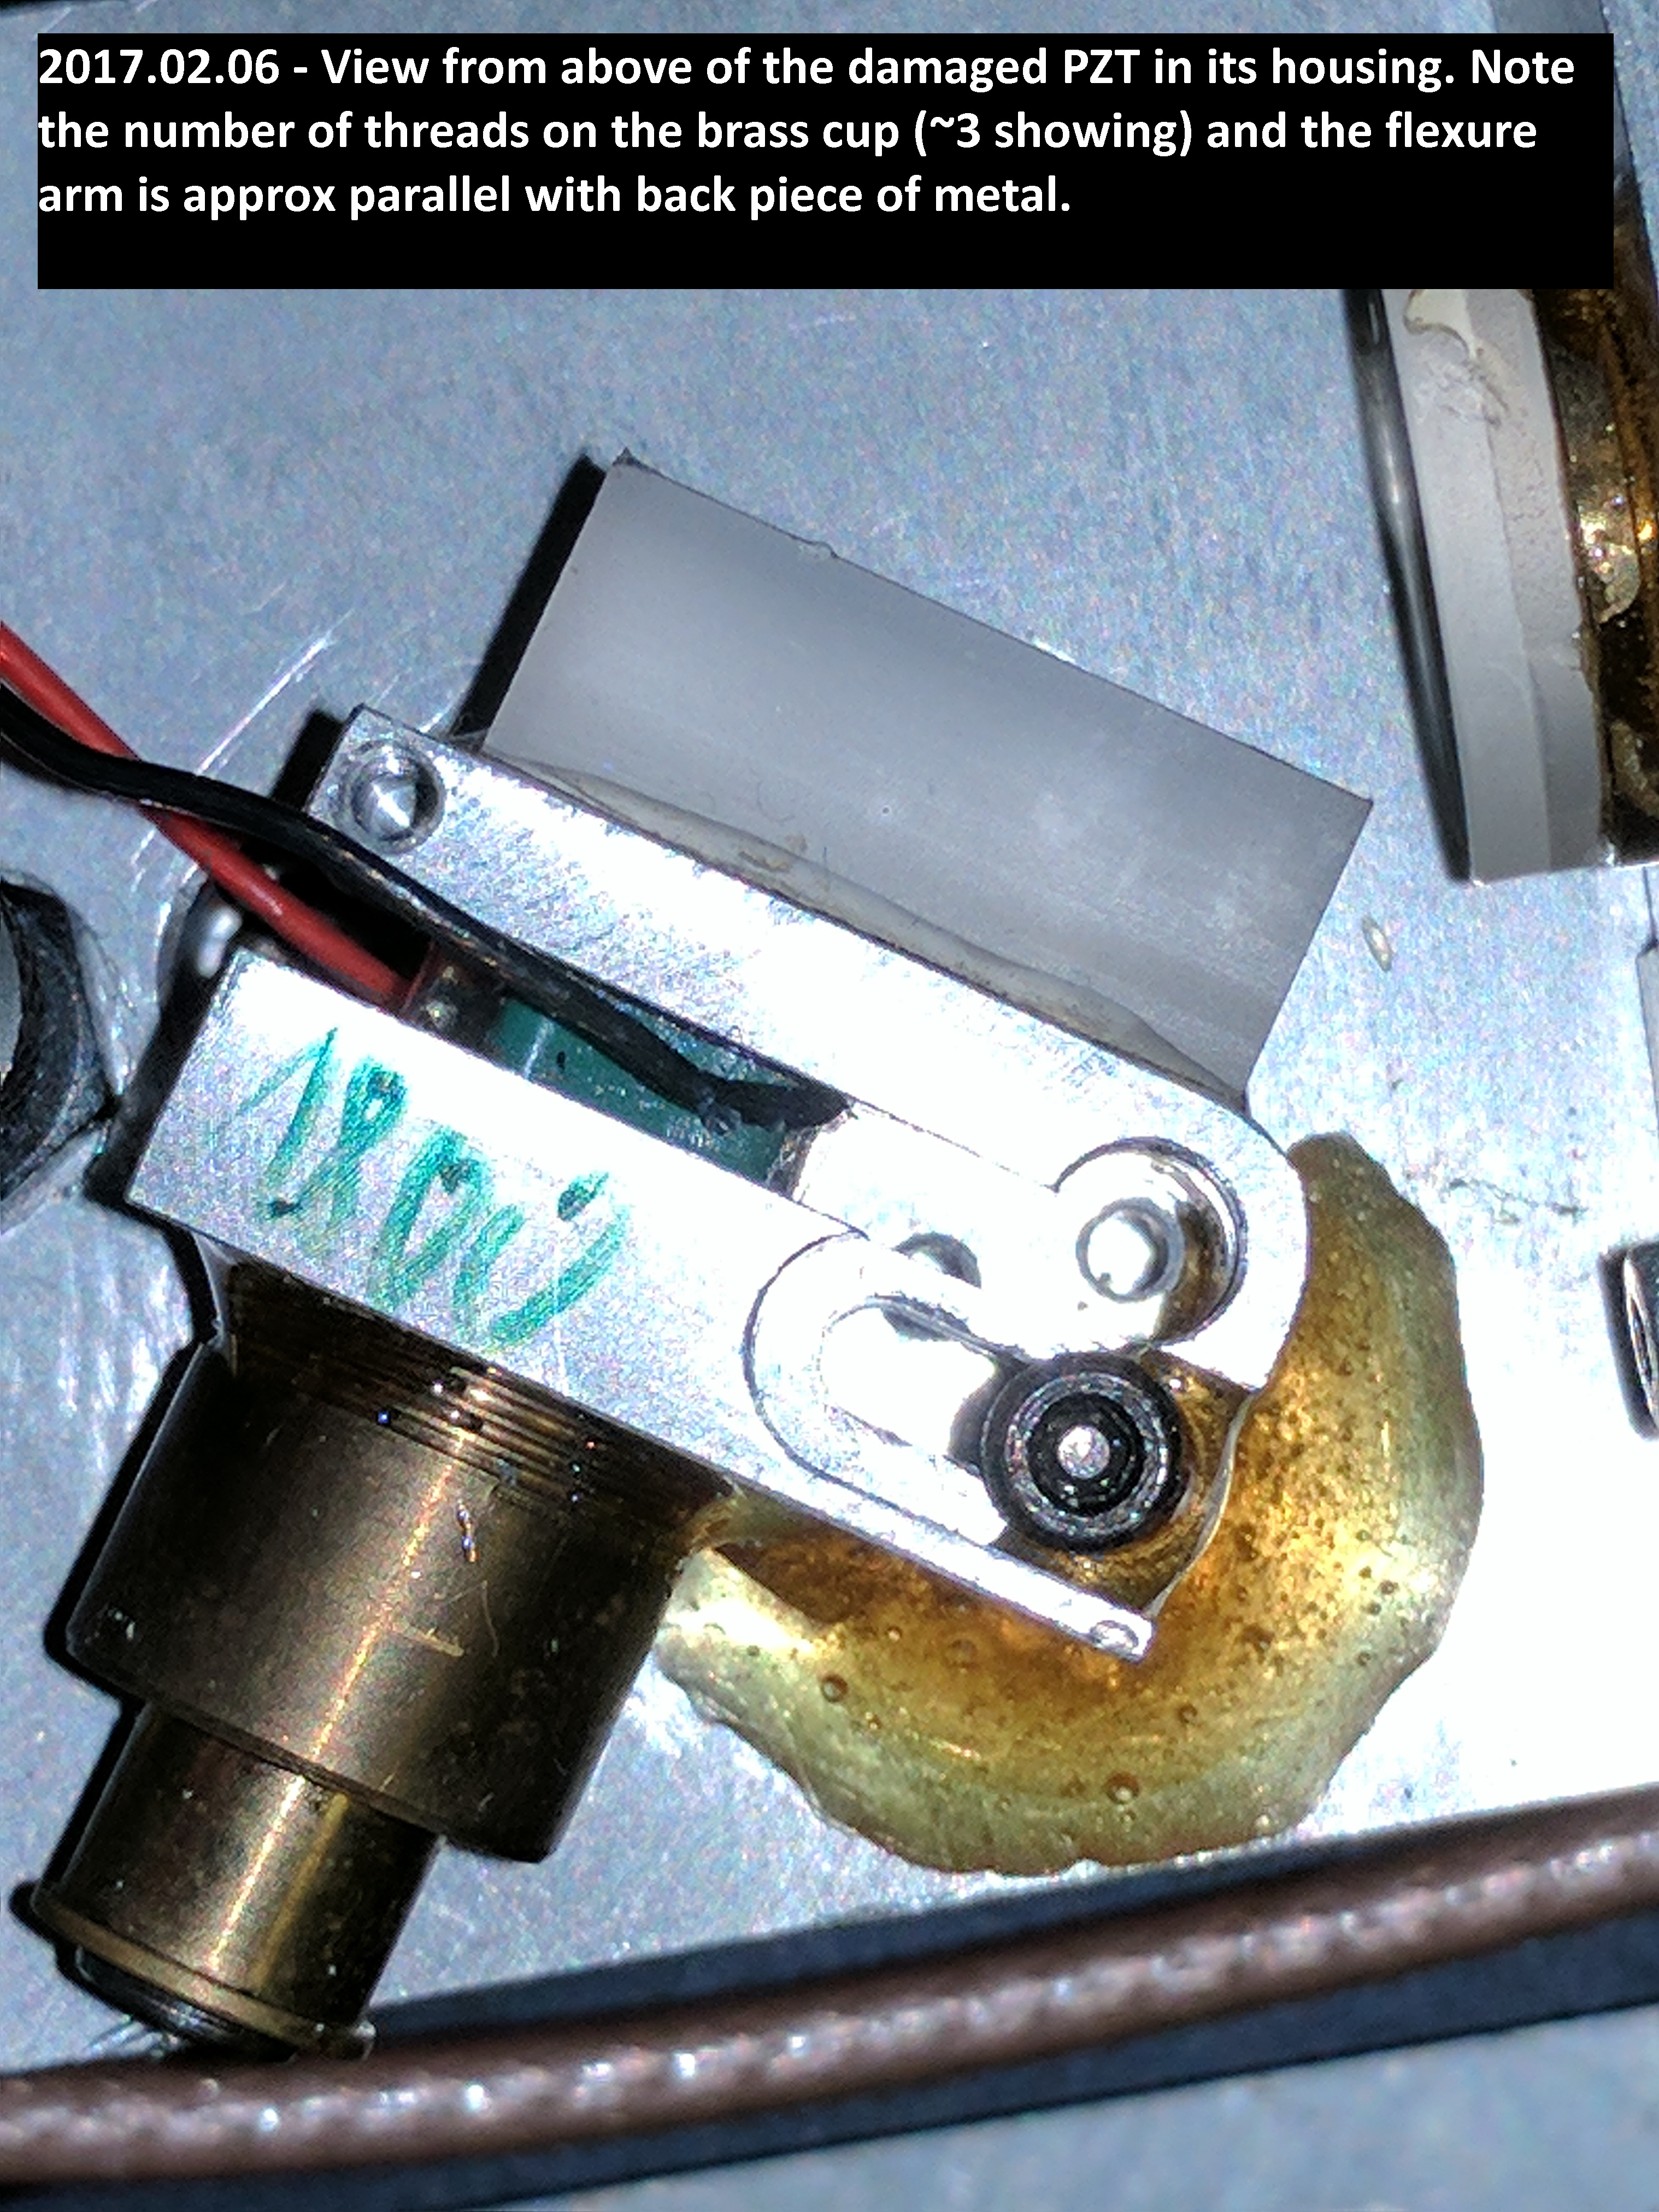
\includegraphics[height=0.4\textheight]{2017.02.06_Damaged PZT_TopView.jpg}}
		\caption{Damaged 922 master PZT}
	\end{figure}
	\begin{figure}
		\centerline{
		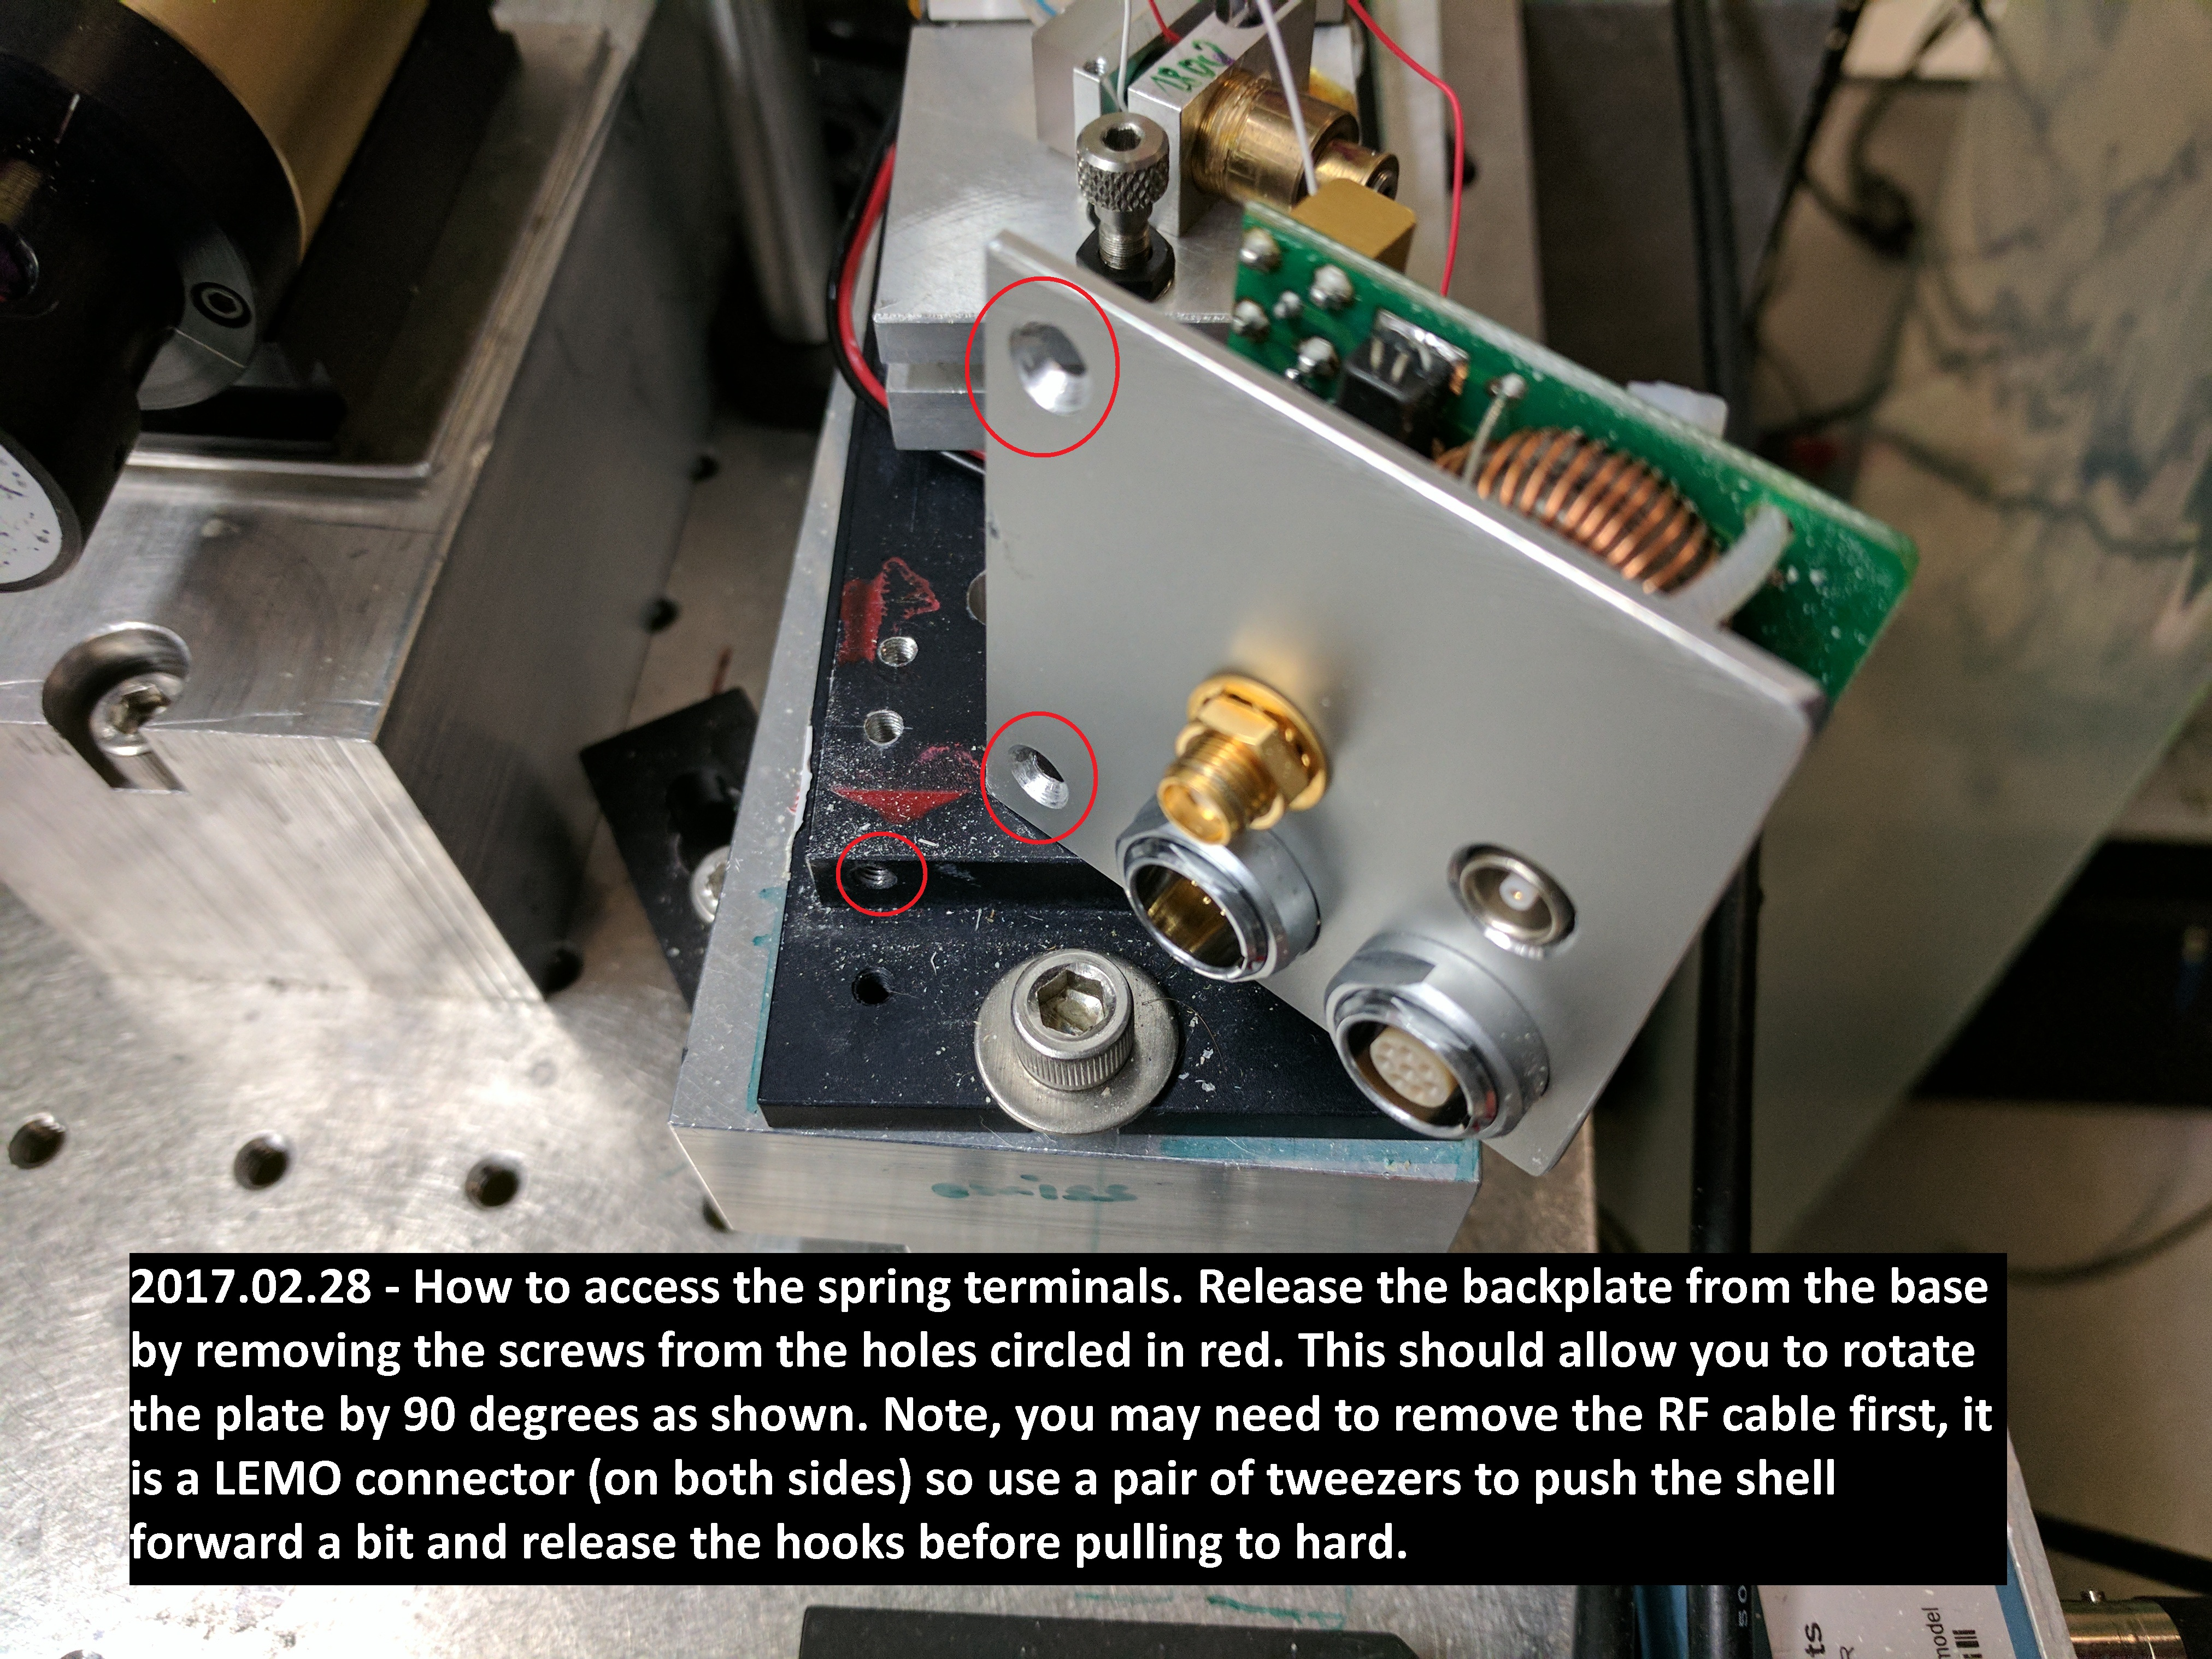
\includegraphics[height=0.4\textheight]{2017.02.28_Step1_RemovingTheCircuitBoard.jpg}}
		\caption{Removing the circuit board of the 922 master}
	\end{figure} 
	\begin{figure}
		\centerline{
		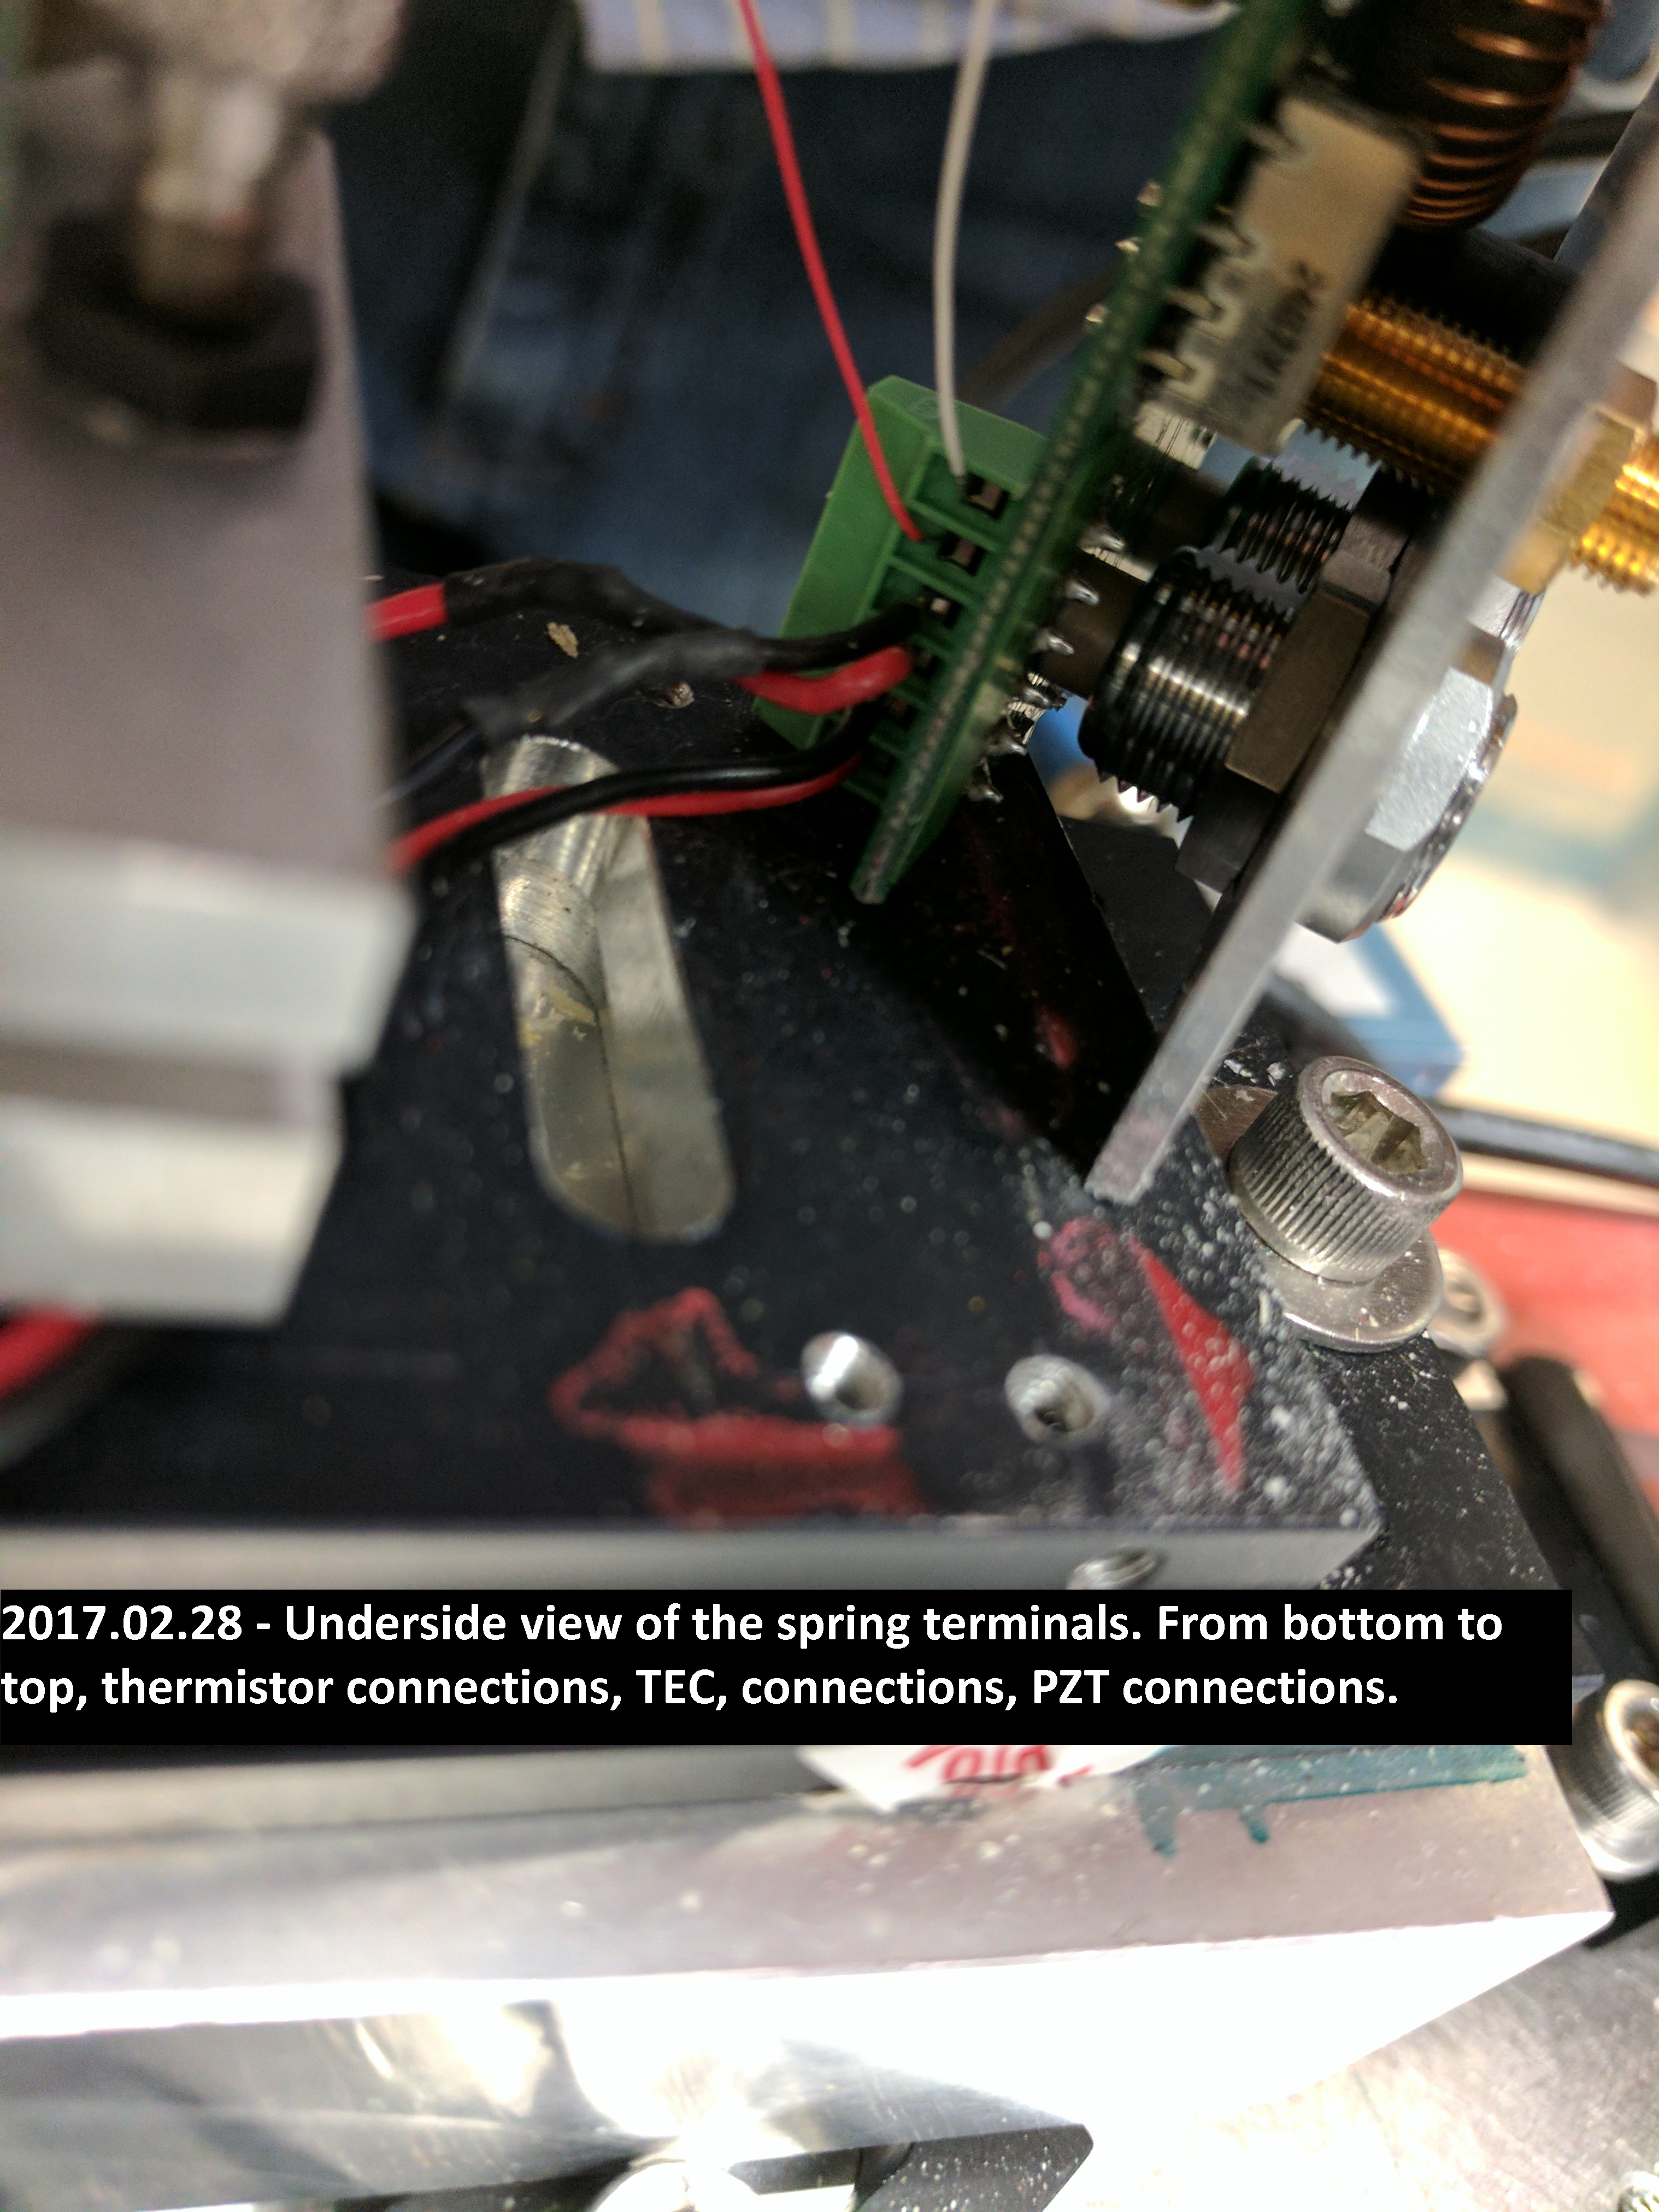
\includegraphics[height=0.4\textheight]{2017.02.28_Step2_ViewOfSpringTerminals.jpg}}
		\caption{Reference image of the spring terminal connections}
	\end{figure} 
	\begin{figure}
		\centerline{
		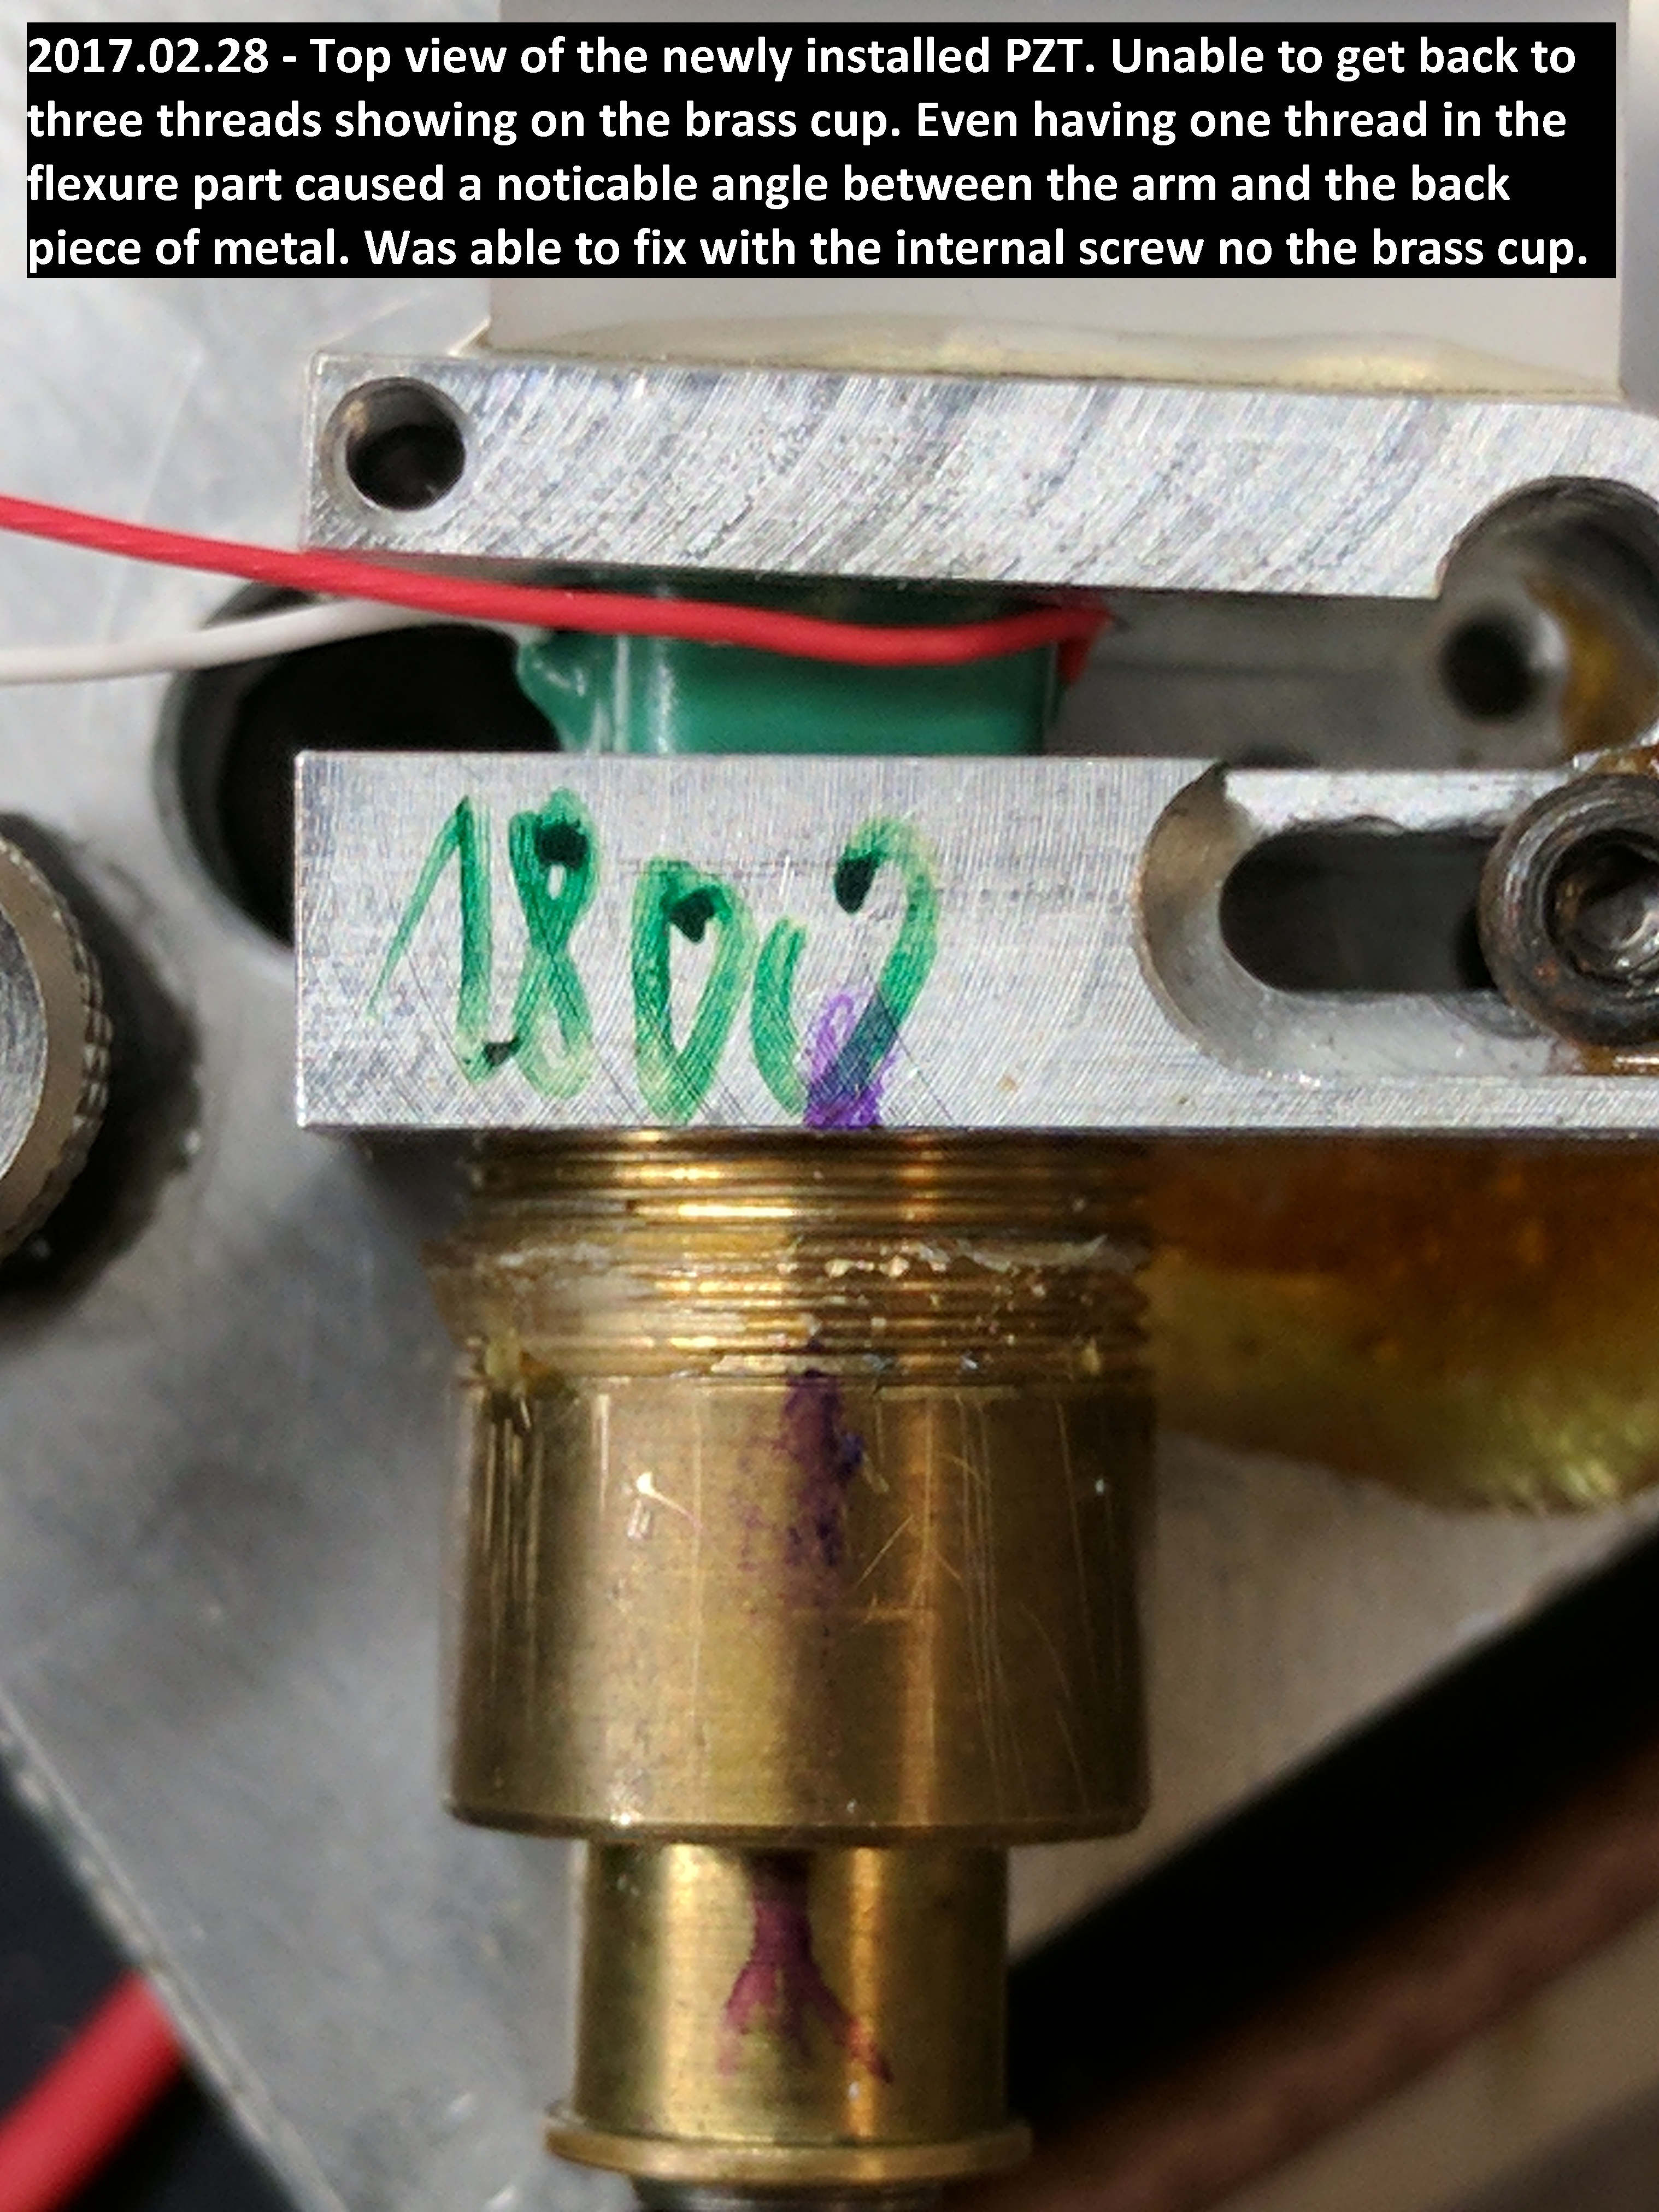
\includegraphics[height=0.4\textheight]{2017.02.28_NewlyInstalledPZT.jpg}}
		\caption{Newly installed 922 master PZT}
	\end{figure}
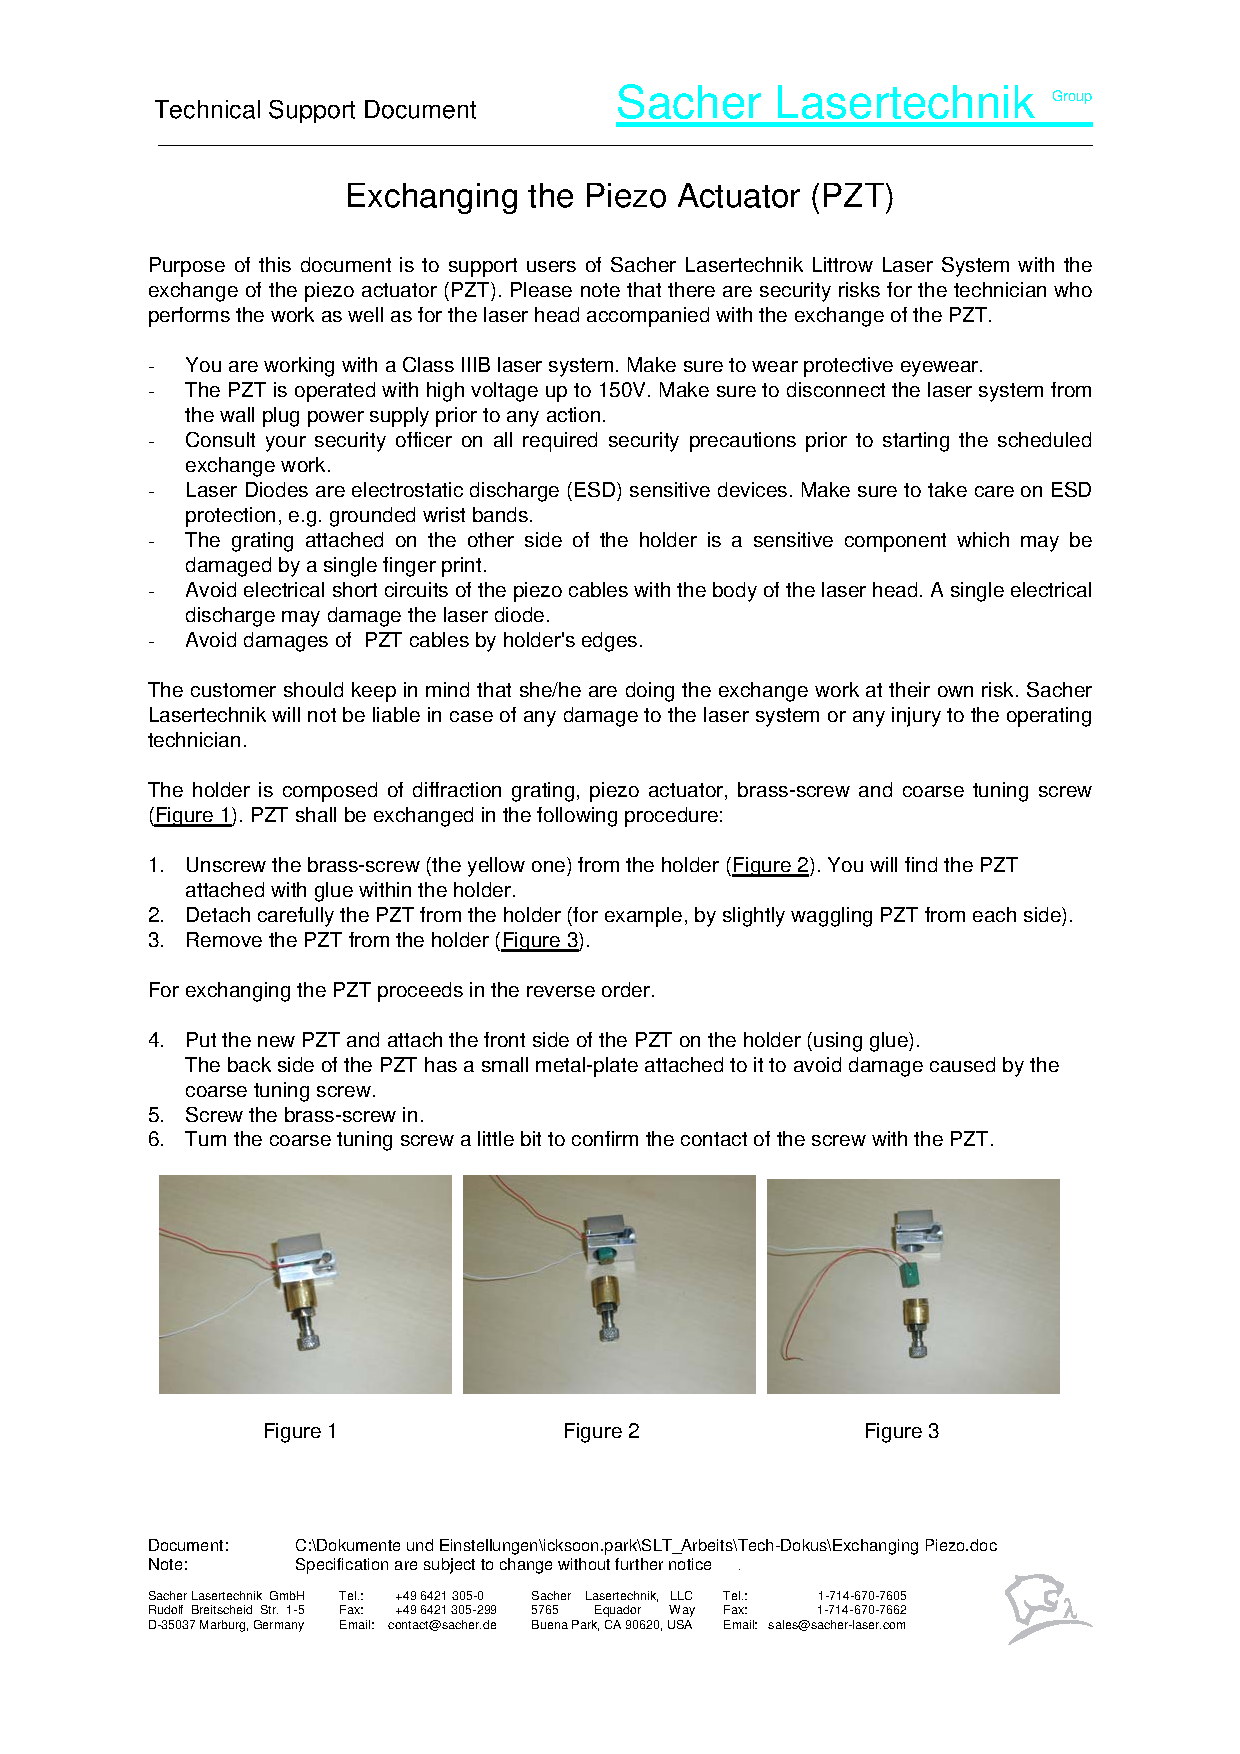
\includepdf[pages=-]{SacherExchangingPiezo.pdf}